\documentclass{article}
\usepackage[margin=1in]{geometry}
\usepackage{amsmath}
\usepackage{listings}
\usepackage{color}
\usepackage{graphicx}
\usepackage{blkarray}
\usepackage{multirow}

\definecolor{dkgreen}{rgb}{0,0.6,0}
\definecolor{gray}{rgb}{0.5,0.5,0.5}
\definecolor{mauve}{rgb}{0.58,0,0.82}

\lstset{frame=tb,
  language=Python,
  aboveskip=3mm,
  belowskip=3mm,
  showstringspaces=false,
  columns=flexible,
  basicstyle={\small\ttfamily},
  numbers=none,
  numberstyle=\tiny\color{gray},
  keywordstyle=\color{blue},
  commentstyle=\color{dkgreen},
  stringstyle=\color{mauve},
  breaklines=true,
  breakatwhitespace=true,
  tabsize=3
}

\begin{document}
\begin{titlepage}
	\setlength{\parindent}{0pt}
	\large

\vspace*{-2cm}

University of Waterloo \par
Econ 424 \par
2023-10-21 \par
\vspace{0.05cm}
Anonymized Usernmae: IJustWannaPass
\vspace{0.2cm}

{\huge Prediction Competition \# 5 \par}
\hrule

\vspace{1cm}
\textbf{Q1)} To solve this problem, I used a variation of boosting. Due to the fact that across k feature space the data could still not be accurately linearly estimated (as shown in Q2), what I did was split the data into buckets. Each bucket would have its own boosted model trained on the data in the bucket. Then I would use a boosted model to create a rough estimate for the price, and determine what bucket to use to get a more accurate measure. Much like the previous prediction contest that means we get the following results:
\[ MSE = 0.06275 \]
\[ R^2 = 0.82178 \]

\textbf{Q2)} Below is a graph showing the difference in price over the distance taken to modulus of 10000. What this does is lets us do is analyse if theres a substantial difference between any of the digits (left most bias) as can be seen on the graph below, the blue shows observations and the red shows average observation value at that modulus value:
\begin{center}
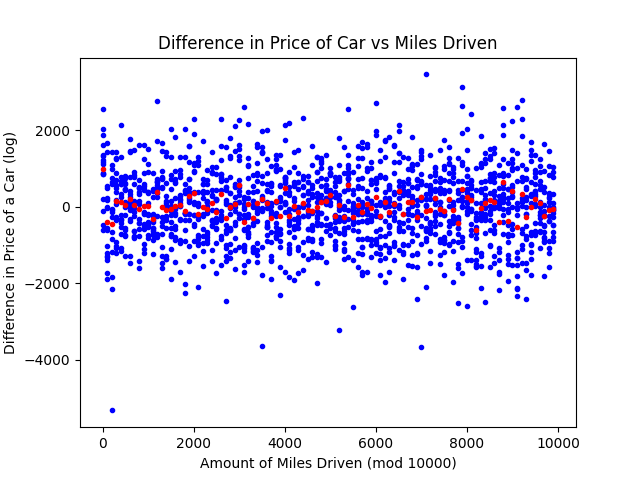
\includegraphics[width=0.8\textwidth]{g3.png}
\end{center}
As we can see, there are spikes that occur before any of the thousands and after the spikes we see the price grow. This can be seen at 4000 and 6000 very easily. This demonstrates the importance of the thousand digit and how consumers far over weigh this. Thus giving us proof of the left bias.
\newpage
\textbf{Q3)} To solve Q1 chatGPT was given the prompt: 
\begin{verbatim}
  Given the same car prediction model, how can I improve predictions for cars that have a cost of a specific threshold. 
\end{verbatim}
chatGPT provided the following response:
\begin{verbatim}
If you want to improve predictions for cars that have a cost around a specific threshold, you can consider the following strategies:

Data Collection and Augmentation:

a. Gather more data specifically for cars around the threshold price. This can help your model better understand the features and characteristics of cars in that price range.

b. Augment your dataset by creating synthetic data points around the threshold price. You can generate variations of existing data points by slightly modifying features or adding noise to mimic cars at the desired price range.

Feature Engineering:

a. Create new features that capture the unique attributes of cars near the threshold price. These features can provide additional information to the model.

b. Explore interactions between features and their effects on cars at the specified price range.

Model Selection and Tuning:

a. Choose a model that is well-suited for capturing the nuances of cars at the threshold price. More complex models or ensemble methods might work better for such specific tasks.

b. Fine-tune hyperparameters, particularly those related to the model's sensitivity to different price ranges.

c. Consider using specialized regression techniques, such as Quantile Regression, that focus on predicting specific quantiles of the target variable. This can be useful when you want to predict a specific threshold price with greater accuracy.

Ensemble Models:

a. Use ensemble models like stacking or blending to combine predictions from multiple models. You can have one model specialized for the specific threshold and another for the rest of the data.

Feature Importance Analysis:

a. Analyze the feature importance scores of your model, which can help identify the features that have the most impact on predictions near the threshold price. This information can guide feature engineering efforts.

Custom Threshold Handling:

a. Implement custom post-processing steps to fine-tune predictions around the threshold price. For example, you can adjust predictions by a certain factor if they are close to the threshold.

Analyze Residuals:

a. Examine the residuals (the differences between actual and predicted values) for cars near the threshold price. This can help identify patterns and systematic errors that your model makes in this price range.

Cross-Validation:

a. Use cross-validation techniques that focus on the threshold price range, such as stratified cross-validation. This ensures that the model's performance in this specific range is adequately assessed during model training and evaluation.

Domain Knowledge:

a. Consult experts or domain-specific knowledge to understand what features and characteristics are most important for cars at the specified price threshold.

Continuous Monitoring and Refinement:

a. Continuously monitor the model's performance, and be prepared to update the model as new data becomes available or as your understanding of the problem improves.

Remember that improving predictions for a specific price threshold might require a combination of these strategies. It's often an iterative process where you experiment, evaluate, and refine your model to achieve the desired level of accuracy around the target price range.
\end{verbatim}
\newpage
To solve Q2 chatGPT was given the prompt:
\begin{verbatim}
   Using a sample dataset how can I demonstrate the impact the most significant digit has on the response variable 
\end{verbatim}
chatGPT provided the following response: 
\begin{verbatim}
To demonstrate the impact of the most significant digit on the response variable, you can use a sample dataset and analyze how the first digit of a numerical feature relates to the response variable. This kind of analysis is commonly associated with Benford's Law, which describes the expected distribution of leading digits in many datasets. You can perform the following steps to demonstrate this impact:

Generate or Prepare a Sample Dataset:
Start by creating or obtaining a sample dataset that includes a numerical feature and a response variable. For simplicity, you can generate a synthetic dataset.

Extract the first digit from the numerical feature. You can do this by converting the numbers to strings and then extracting the first character.

Aggregate and Analyze the Data:
Calculate summary statistics for the response variable based on the first digit of the numerical feature. You can calculate the mean, median, or other relevant statistics for each first digit group. This analysis helps you understand how the first digit affects the response variable.

Visualize the Impact:
Create visualizations to demonstrate the impact of the first digit. You can create bar plots, histograms, or box plots to show how the response variable varies with the first digit.

Interpret the Results:
Analyze the results to determine if there is a notable impact of the first digit on the response variable. You can look for patterns or differences in means or other statistics across different first digits.

The analysis demonstrates how the first digit of the numerical feature affects the response variable and whether it follows any expected patterns, such as those outlined in Benford's Law. If the first digit has a significant impact on the response variable, it may suggest that the numerical feature follows a particular distribution or that other factors are influencing the relationship.
\end{verbatim}
\end{titlepage}
\textbf{Code for Q1:}
\begin{lstlisting}
import matplotlib.pyplot as plt
import numpy as np
import pandas as pd
import xgboost as xgb
import warnings
from pandas.util import hash_pandas_object

warnings.filterwarnings("ignore")
from sklearn.model_selection import train_test_split
from sklearn.neighbors import KNeighborsClassifier

# Read in the data
data = pd.read_csv("Econ424_F2023_PC4_training_data_large.csv", low_memory=False)

# Keep only the most relevant stats
data = data.loc[:,
       data.columns.intersection(['price', 'model_name', 'mileage', 'daysonmarket', 'owner_count', 'year'])]
# If owner_count is empty assume its 0
data["owner_count"] = data["owner_count"].fillna(0)
# Drop empty columns
data.dropna(inplace=True)
# Standardize results
data["price"] = data["price"].map(lambda x: np.log(x))
data["mileage"] = data["mileage"].map(lambda x: np.log(int(x) + 1))

# ===================== Data Processing =====================
# assign each value to a dict
modelDict = {}


def classify(model):
    if model not in modelDict:
        modelDict[model] = len(modelDict)


data.apply(lambda x: classify(x['model_name']), axis=1)
data["model_name"] = data["model_name"].map(lambda x: modelDict[x])

# We will now define 3 buckets dependent on the price of the car, such that if we estimate a car to be in a specific
#  range we will use the bucket estimate instead of the overall estimator.
data.sort_values(by=['price'], inplace=True, ignore_index=True)

numberOfBuckets = 11
numberOfEntries = len(data)
markers = [data.iloc[0, 0]]
adjustment = np.abs((data.iloc[0, 0] - data.iloc[numberOfEntries - 1, 0]) / 14)
for i in range(1, numberOfBuckets + 1):
    if i == numberOfBuckets:
        markers.append(data.iloc[numberOfEntries - 1, 0])
    else:
        markers.append(data.iloc[int(i * numberOfEntries / numberOfBuckets), 0])

# We will then train classifiers with data a little past each marker
modelArr = []
for bucket in range(0, numberOfBuckets):
    if bucket == numberOfBuckets - 1:
        slice = data[(data['price'] > markers[bucket] - adjustment) & (data['price'] <= markers[bucket + 1])]
    elif bucket == 0:
        slice = data[(data['price'] >= markers[bucket]) & (data['price'] <= markers[bucket + 1] + adjustment)]
    else:
        slice = data[
            (data['price'] > markers[bucket] - adjustment) & (
                    data['price'] <= markers[bucket + 1] + adjustment)]

    innerModel = xgb.XGBRegressor(n_estimators=500, max_depth=4, eta=0.1, subsample=0.7, colsample_bytree=0.8)
    x = slice.iloc[:, 1:]
    y = slice.iloc[:, 0]
    innerModel.fit(x, y)
    modelArr.append(innerModel)

print(markers)


# ===================== Data Testing =====================

def getModelName(modelName):
    if modelName in modelDict:
        return modelDict[modelName]
    return 0


# Read in the test data and modify the data
test = pd.read_csv("Econ424_F2023_PC5_test_data_without_response_var.csv", low_memory=False)
test["owner_count"] = test["owner_count"].fillna(0)
test = test.interpolate()
test = test.loc[:,test.columns.intersection(['model_name', 'mileage', 'daysonmarket', 'owner_count', 'year'])]
test["model_name"] = test["model_name"].map(lambda x: getModelName(x))
test["mileage"] = test["mileage"].map(lambda x: np.log(int(x) + 1))

# Start by predicting using a regular classifier, based of results use a more specific classifier
baseLine = xgb.XGBRegressor(n_estimators=500, max_depth=4, eta=0.1, subsample=0.7, colsample_bytree=0.8)
x = data.iloc[:, 1:]
y = data.iloc[:, 0]
baseLine.fit(x, y)
prediction_base = baseLine.predict(test)
test["predicted_base_price"] = prediction_base
test['New_ID'] = test.index


pred = {}
# Using the old predictions, use the buckets to predict again
for bucket in range(0, numberOfBuckets):
    print(bucket)
    if bucket == numberOfBuckets - 1:
        slice = test[test['predicted_base_price'] > markers[bucket]]
    elif bucket == 0:
        slice = test[test['predicted_base_price'] <= markers[bucket + 1]]
    else:
        slice = test[
            (test['predicted_base_price'] > markers[bucket]) & (
                    test['predicted_base_price'] <= markers[bucket + 1])]

    slice.reset_index()
    loctest = slice.iloc[:, 0:-2]
    loctest.reset_index()
    predicted = modelArr[bucket].predict(loctest)

    for idx in range(0, len(predicted)):
        key = slice.iloc[idx, -1]
        pred[key] = predicted[idx]



# ===================== Export Model =====================

test["predicted_spec_price"] = test.apply(lambda x: pred[x.loc['New_ID']], axis=1)
val = test["predicted_spec_price"]

f = open('predictions.csv', 'w')
for estimate in val:
    f.writelines(str(estimate) + ",\n")

\end{lstlisting}
\end{document}